% ju 03-Okt-22
\documentclass[a4paper,12pt,fleqn,parskip=half]{scrartcl}
\usepackage[ngerman]{babel}
\usepackage[utf8]{inputenc}
\usepackage[T1]{fontenc}

% Schrift
%\usepackage{lmodern}
\usepackage[osf,sc]{mathpazo} 
\usepackage[scale=.9,semibold]{sourcecodepro}   
\usepackage[osf]{sourcesanspro}  

\usepackage[headsepline]{scrlayer-scrpage}
\pagestyle{scrheadings}
\clearpairofpagestyles

\usepackage[table,dvipsnames,usenames]{xcolor}
\usepackage{textcase}
\usepackage{nameref}
\usepackage{hyperref}
\usepackage{tabularx}
\usepackage{multirow}
\usepackage{multicol}
\usepackage{caption, booktabs}
\usepackage{graphicx} 
\usepackage{scrhack}    
\usepackage{url}%% Links
\usepackage[inline]{enumitem}
\usepackage{pifont}
\usepackage{eurosym}% \euro 20,-
\usepackage{amsmath}
\usepackage{amsfonts}
\usepackage{amssymb}
\usepackage{array}            % Extending the array and tabular environments
\usepackage{chngcntr}         % Change the resetting of counters
\usepackage[version=4]{mhchem}
\usepackage{stmaryrd}
\usepackage{siunitx}
\usepackage{float}
\usepackage{csquotes}
\usepackage{subcaption}
\usepackage{mathtools}
\usepackage{icomma}%Dezimaltrennzeichen
\usepackage{multimedia}%Video: \movie[externalviewer]{(video.mov)}{video.mov}
\usepackage{epstopdf}
\usepackage{footnote}
\usepackage{qrcode}% Anwendung: \qrcode[hyperlink,level=Q,version=2,height=1cm]{\website}
\usepackage{underscore}% Unterstrich ____

% PDF Dokumente einbinden
\usepackage{pdfpages}% \includepdf[pages=-]{Tabellen/Excel.pdf}
\RequirePackage{lastpage}  % Pagecounter

\addto\captionsngerman{%
\renewcommand{\figurename}{Abb.}
\renewcommand{\tablename}{Tab.}
}

% listings
\usepackage{listings}
\lstset{basicstyle=\linespread{1}\ttfamily\small,floatplacement=!htb,captionpos=t,abovecaptionskip=.5\baselineskip,belowcaptionskip=.5\baselineskip,upquote=true,showstringspaces=false,inputencoding=utf8,tabsize=4,
    	keywordstyle=\bfseries ,
	commentstyle=\color{rot5},
	stringstyle=\color{orange},
	breaklines=true,
  	postbreak=\mbox{\textcolor{black}{$\hookrightarrow$}\space},
	breakatwhitespace=false
}
\lstset{literate={á}{{\'a}}1 {é}{{\'e}}1 {í}{{\'i}}1 {ó}{{\'o}}1 {ú}{{\'u}}1 {Á}{{\'A}}1 {É}{{\'E}}1 {Í}{{\'I}}1 {Ó}{{\'O}}1 {Ú}{{\'U}}1 {à}{{\`a}}1 {è}{{\`e}}1 {ì}{{\`i}}1 {ò}{{\`o}}1 {ù}{{\`u}}1 {À}{{\`A}}1 {È}{{\'E}}1 {Ì}{{\`I}}1 {Ò}{{\`O}}1 {Ù}{{\`U}}1 {ä}{{\"a}}1 {ë}{{\"e}}1 {ï}{{\"i}}1 {ö}{{\"o}}1 {ü}{{\"u}}1 {Ä}{{\"A}}1 {Ë}{{\"E}}1 {Ï}{{\"I}}1 {Ö}{{\"O}}1 {Ü}{{\"U}}1 {â}{{\^a}}1 {ê}{{\^e}}1 {î}{{\^i}}1 {ô}{{\^o}}1 {û}{{\^u}}1 {Â}{{\^A}}1 {Ê}{{\^E}}1 {Î}{{\^I}}1 {Ô}{{\^O}}1 {Û}{{\^U}}1 {œ}{{\oe}}1 {Œ}{{\OE}}1 {æ}{{\ae}}1 {Æ}{{\AE}}1 {ß}{{\ss}}1 {ű}{{\H{u}}}1 {Ű}{{\H{U}}}1 {ő}{{\H{o}}}1 {Ő}{{\H{O}}}1 {ç}{{\c c}}1 {Ç}{{\c C}}1 {ø}{{\o}}1 {å}{{\r a}}1 {Å}{{\r A}}1 {€}{{\EUR}}1 {£}{{\pounds}}1 {~}{{\textasciitilde}}1 {-}{{-}}1 }

% bibliography
\usepackage[
    bibencoding=utf8,
    backend=biber,% bibtex, biber
    backref=false,backrefstyle=three+,url=true,urldate=comp,abbreviate=false,maxnames=20
]{biblatex} %Paket laden
\DeclareBibliographyCategory{cited}
\let\defaultcite\cite\renewcommand*\cite[2][]{\addtocategory{cited}{#2}\defaultcite[#1]{#2}}
\let\defaulttextcite\textcite\renewcommand*\textcite[2][]{\addtocategory{cited}{#2}\defaulttextcite[#1]{#2}}
\setcounter{biburllcpenalty}{7000}
\setcounter{biburlucpenalty}{8000}
\AfterPackage{biblatex}{
	\PreventPackageFromLoading[\errmessage{Sie haben versucht, das Cite-Paket zu laden, das nicht mit biblatex kompatibel ist.}]{cite}
}

\hypersetup{%
	%pdftitle={\titel},
	%pdfsubject={Latex},
	%pdfauthor={\autor},
	%pdfcreator={\autor}, 
	bookmarksnumbered=true,
	breaklinks=true,
	%colorlinks=true,	   
	linkcolor=rot5,		
	filecolor=blau5,		
	urlcolor=blau5,			
	citecolor=ForestGreen
}

\linespread{1.1}
\setlist{itemsep=0pt}
\widowpenalty10000
\clubpenalty10000
\tolerance1000   

\usepackage[left=2cm,right=2cm,top=1cm,bottom=1cm,includeheadfoot]{geometry}
%\usepackage[left=4cm,right=2cm,top=1cm, bottom=1cm,includeheadfoot]{geometry}
%\usepackage[left=6cm,right=1cm,top=1cm, bottom=1cm,includeheadfoot]{geometry}
%\usepackage[landscape=true,left=2cm,right=2cm,top=1cm,bottom=1cm,includeheadfoot]{geometry}%quer

% eigene Farbe definieren
% Adobe Prozessfarben: CMYK: 100,50,0,35 -> 1,0.5,0,0.35
\definecolor{orange}{cmyk}{0,0.55,0.61,0}   % 0,55,61,0
\definecolor{blau5}{cmyk}{1,0.77,0.1,0.01}  % 100,77,10,
\definecolor{rot5}{cmyk}{0.22,1,1,0.19}     % 22,100,100,19
\definecolor{grau2}{cmyk}{0,0,0,0.1}        % 0,0,0,40
\definecolor{blau}{cmyk}{0.93,0.66,0,0.21}% 

% Literatur
\bibliography{content/literatur}
\bibliography{content/literatur-kfz}
\bibliography{content/literatur-sport}

%%%%%%%%%%%%%%%%%%%%%%%%%%%%%%%%%%%%%%%%%%%%%%%%%%%%%%%
\newcommand{\name}{Jan Unger}
\newcommand{\thema}{09-Common-Rail-Einspritzung}
\newcommand{\quelle}{\name}
\newcommand{\website}{https://bw-ju.de/}
\newcommand{\github}{https://github.com/ju1-eu}
%%%%%%%%%%%%%%%%%%%%%%%%%%%%%%%%%%%%%%%%%%%%%%%%%%%%%%%

\ihead{\textbf{Quelle:} \quelle}%{Kopfzeile innen}
\ohead{\textbf{Datum:} \today}  %{Kopfzeile außen}
\ifoot{\textbf{Thema:} \thema}  %{Fußzeile  innen}
\ofoot{Seite {\thepage} von {\pageref{LastPage}}}%{Fußzeile  außen}

\title{\thema}
\author{\name}
\date{\today}

\begin{document}
	%%%%%%%%%%%%%%%%%%%%%%%%%%%%%%%%%%%%%%%%%%%%%%%%%%%%%%%%%%%%%%%%%%
	\begin{abstract}
		\center
		\textbf{\Large \thema}%14pt
		
		\vspace{1.5em}
		%\datum	
		%\qrcode[hyperlink,level=Q,version=2,height=1cm]{\website}
		\qrcode[hyperlink,level=Q,version=2,height=1cm]{\github}
		
		\vspace{1.5em} 
		\raggedright
		\textbf{\large Keywords}
		% Checkliste
		\begin{itemize}[label=\checkmark]
			\item Begriff
		\end{itemize}
	\end{abstract}
    %%%%%%%%%%%%%%%%%%%%%%%%%%%%%%%%%%%%%%%%%%%%%%%%%%%%%%%%%%%%%%%%%%

	% anpassen
	%\input{content/tex/neu}
	%ju 17-Sep-22 09-Common-Rail-Einspritzung.tex
\begin{figure}[!ht]% hier: !ht
\centering
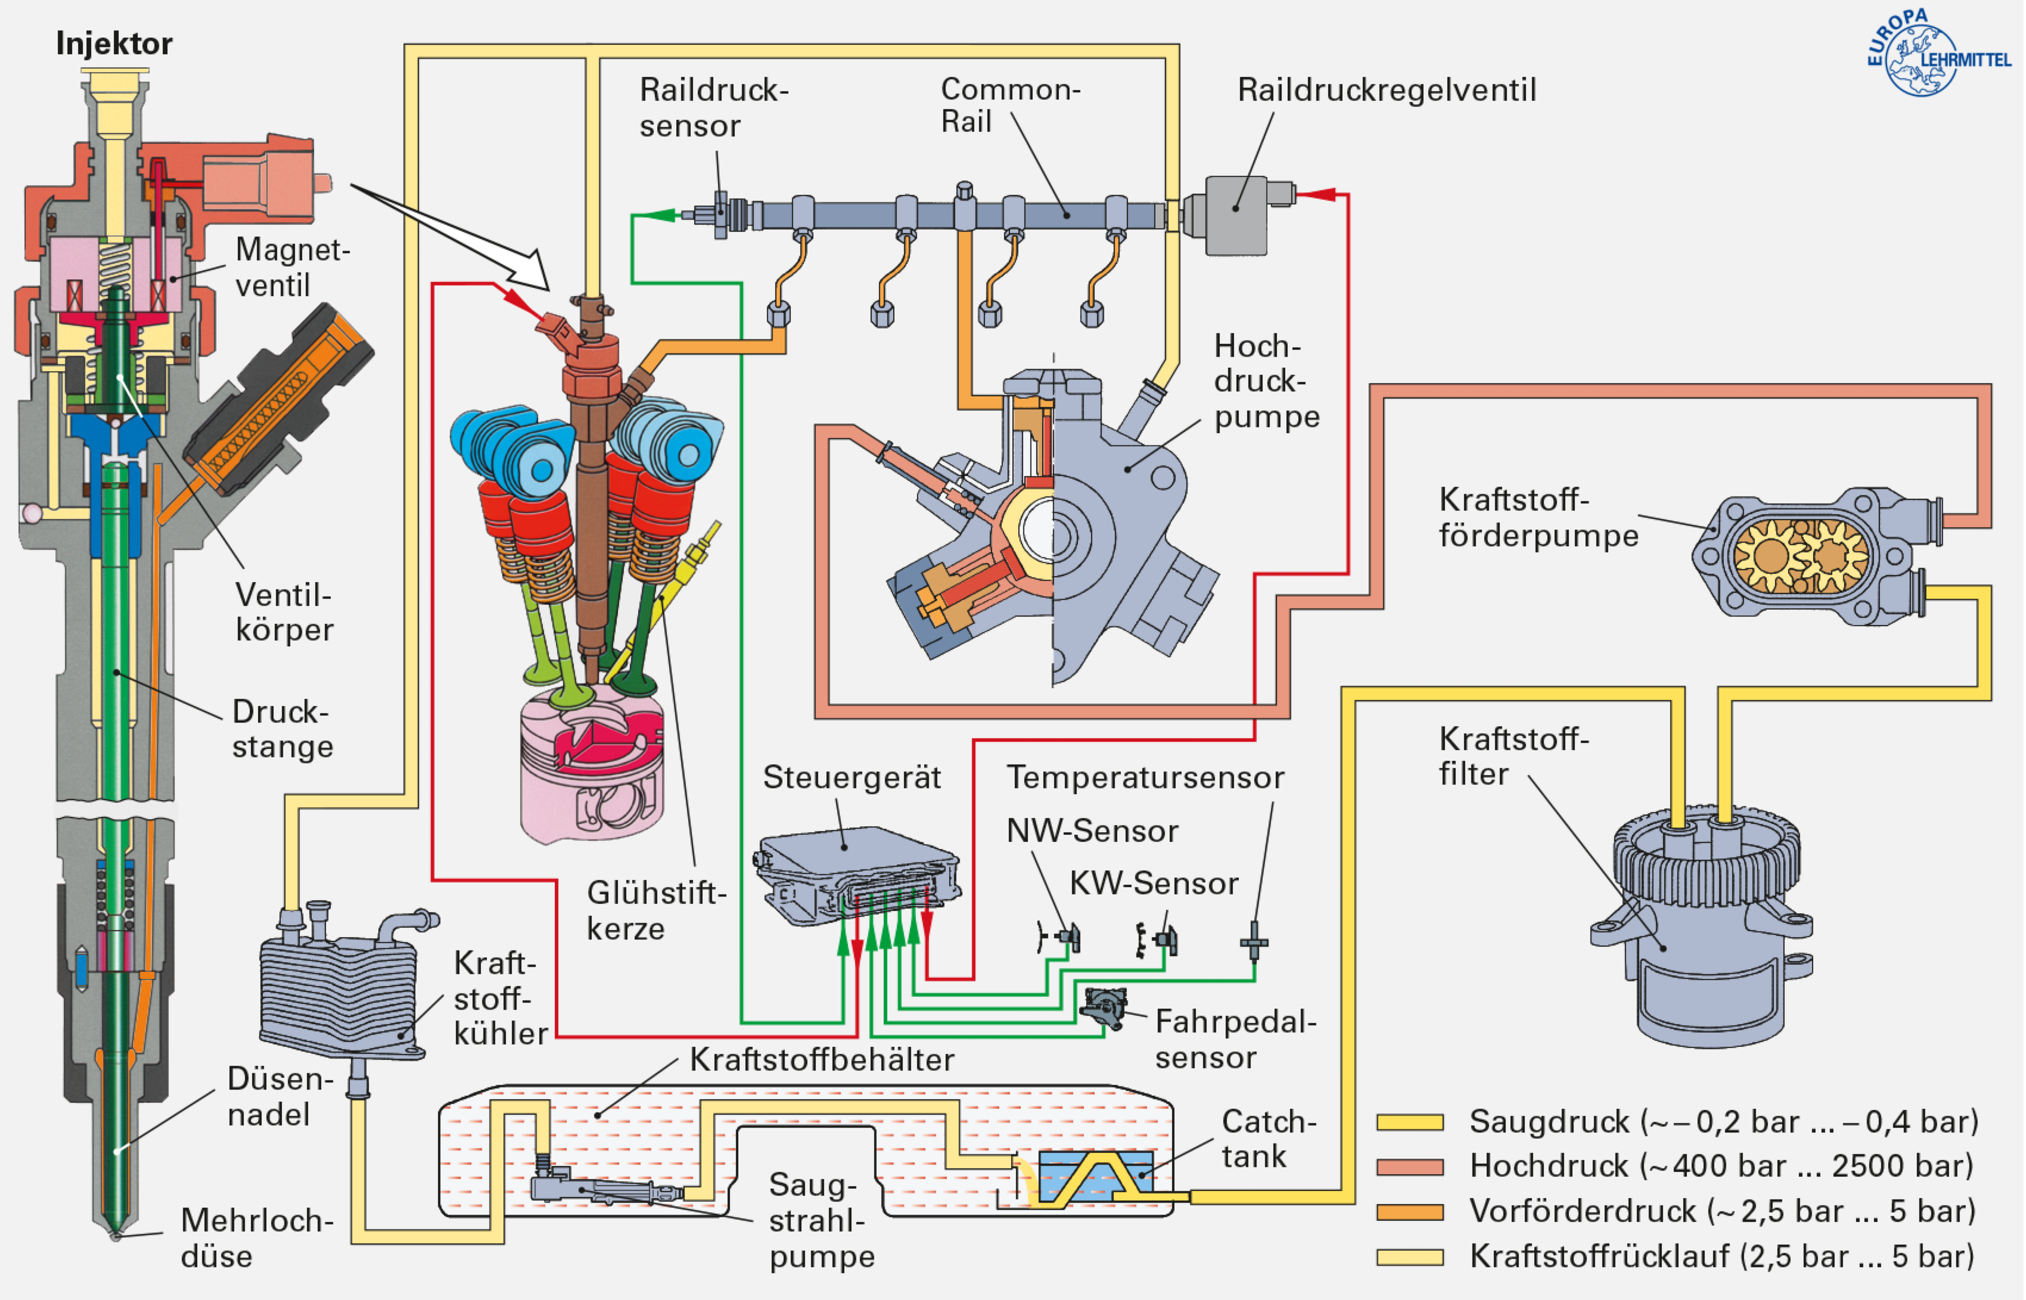
\includegraphics[width=0.7\textwidth]{images/CR/Common-Rail.png}
\caption{Common Rail, Quelle: Europa-Verlag SimKfz}
%\label{fig:}%% anpassen
\end{figure}

\textbf{Bauteile und Aufgaben}

\begin{enumerate}
\item
  \textbf{Elektrische Kraftstoffpumpe} Kraftstoff zu Hochdruckpumpe
  fördern.
\item
  \textbf{Hochdruckpumpe} Kraftstoff unter Hochdruck in das Rail
  fördern.
\item
  \textbf{Rail} Hochdruck speichern und Verteilung des Kraftstoffs auf
  die Injektoren.
\item
  \textbf{Druckregelventil} den erforderlichen Hochdruck an jeden
  Betriebszustand anpassen.
\item
  \textbf{Raildrucksensor} Hochdruck erfassen und als elektrisches
  Signal an das Steuergerät weiterleiten.
\item
  \textbf{Injektor} Kraftstoff dosiert in den Brennraum spritzen
\end{enumerate}

\textbf{Welche Ursachen kommen für den Leistungsverlust infrage?}

\begin{enumerate}
\item
  \textbf{Mechanische Fehler}

  \begin{itemize}
  \item
    Kompressionsverlust durch Verschleiß der Ventile oder des Kolbens
  \item
    Verschleiß der Hochdruckpumpe
  \end{itemize}
\item
  \textbf{Fehler im hydraulischen System}

  \begin{itemize}
  \item
    Undichtigkeit an Injektoren (schließt nicht korrekt, tropft nach,
    Düse ausgewaschen)
  \item
    Undichte Leitungen am Rail
  \end{itemize}
\item
  \textbf{Elektrische Fehler}

  \begin{itemize}
  \item
    Sensoren defekt
  \item
    Aktoren defekt
  \item
    Leitungsunterbrechung
  \item
    Masseschluss
  \end{itemize}
\end{enumerate}

\textbf{Laufruheregelung}, die einzelnen Zylinder bekommen mehr oder
weniger Kraftstoff vom Steuergerät zugeteilt.

\textbf{Was muss beachtet werden beim Einbau eines neuen Injektors?}

\begin{itemize}
\item
  Fertigungstoleranz: muss im Steuergerät einprogrammiert werden
\item
  Zahlen- und Buchstabencodes auf dem Injektor
\item
  Steuergerät korrigiert entsprechend die Grundeinspritzmenge des
  jeweiligen Injektors.
\end{itemize}

\textbf{Erkläre den Spannungs- bzw. Stromverlauf eines intakten
Injektors}

\begin{itemize}
\item
  Injektorspannung beträgt in der Anzugsphase ca. 80 V. Der Anzugstrom
  liegt dadurch bei ca. 20 A. Danach wird der Strom auf ca. 12 A
  begrenzt (Haltestrom), bei einer Spannung von 12 V bis 14 V.
\end{itemize}

\textbf{Wie entsteht die Injektorsspannung von 80 bis 100 V?}

\begin{itemize}
\item
  Beim Ausschalten der Magnetventile wird die entstehende
  Induktionsspannung genutzt, um im Steuergerät einen Kondensator
  aufzuladen.
\end{itemize}

\newpage

\textbf{Welche Druckregelungsarten gibt es?}

\begin{enumerate}
\item
  \textbf{Einsteller-Regelung}

  \begin{itemize}
  \item
    \textbf{Druckregelung hochdruckseitig} (Druckregelung)

    \begin{itemize}
    \item
      Hochdruckpumpe fördert die maximale Fördermenge unabhängig von
      Bedarf an Kraftstoff
    \item
      Raildruck wird über ein Druckregelventil geregelt, nicht
      benötigter Kraftstoff fließt zurück in den Tank
    \item
      \textbf{Nachteil:} Hochdruckpumpe ist konstant maximal belastet,
      dadurch

      \begin{itemize}
      \item
        geringere Nutzleistung
      \item
        erhöhter Kraftstoffverbrauch, Schadstoffausstoß, Verschleiß
      \item
        unnötige Erwärmung des Kraftstoffs
      \end{itemize}
    \end{itemize}
  \item
    \textbf{Druckregelung niederdruckseitig} (Mengenregelung)

    \begin{itemize}
    \item
      Raildruck wird über eine Zumesseinheit an der Hochdruckpumpe
      niederdruckseitig geregelt
    \item
      Bedarfsregelung es gelangt nur so viel Kraftstoff zu
      Hochdruckpumpe wie benötigt wird für die Einspritzung
    \item
      Zumesseinheit regelt die Zuflussmenge zur Hochdruckpumpe

      \begin{itemize}
      \item
        Mengenregelventil unbestromt: voll offen für maximale
        Fördermenge
      \item
        Mengenregelventil bestromt: verringert den Öffnungsquerschnitt
        für minimale Fördermenge\\
      \end{itemize}
    \item
      Druckbegrenzungsventil verhindert zu hohen Raildruck bei Ausfall
      der Zumesseinheit
    \item
      \textbf{Nachteil:}

      \begin{itemize}
      \item
        hohe Trägheit
      \item
        Drucksteigerung erfordert zunächst eine Erhöhung des
        Niederdrucks, dadurch erhöhte Förderleistung der Hochdruckpumpe
      \end{itemize}
    \end{itemize}
  \end{itemize}
\item
  \textbf{Zweisteller-Regelung} (\textbf{Druckregelung nieder- und
  hochdruckseitig})

  \begin{itemize}
  \item
    \textbf{Vorteil}

    \begin{itemize}
    \item
      geringe Leistungsaufnahme der Hochdruckpumpe bei konstant hohen
      Drücken
    \item
      hohe Agilität bei geringen Drücken
    \end{itemize}
  \item
    \textbf{Motorstart und Warmlaufphase} hochdruckseitig geregelt

    \begin{itemize}
    \item
      Kraftstoff soll sich erwärmen und damit fließ- und zündfähiger zu
      machen
    \end{itemize}
  \item
    \textbf{betriebswarmer Motor: Leerlauf / Teillast}
    Zweisteller-Betrieb

    \begin{itemize}
    \item
      große Sprünge des Raildrucks sind wahrscheinlich (Motor im
      Leerlauf / Teillast $\to$ Lastwunsch des Fahrers: Volllast)
    \end{itemize}
  \item
    \textbf{hohen Motorlast} niederdruckseitig geregelt

    \begin{itemize}
    \item
      große Steigerungen des Raildrucks nicht möglich und deshalb ist
      die Trägheit vernachlässigbar
    \end{itemize}
  \end{itemize}
\end{enumerate}

\textbf{Druckregelventil} Druckerfassung durch Membransensor am Rail
(Raildrucksensor)

Ansteuerung: PWM-Signal (Raildruck wird größer, wenn Tastverhältnis
größer wird), wenn Magnetventil bestromt: dadurch wird die Schließkraft
der Ventilnadel erhöht oder gesenkt. Dementsprechend wird der Raildruck
erhöht oder gesenkt.

\begin{enumerate}
\item
  \textbf{unbestromt / stromlos} Raildruck etwa $100~\text{bar}$

  \begin{itemize}
  \item
    Motor abstellen, Ventilfeder hält Druckregelventil geschlossen,
    verhindert ein Leerlaufen des Rails
  \end{itemize}
\item
  Magnetventil bestromt, Lastzustände:

  \begin{itemize}
  \item
    \textbf{Motorstart} Raildruck $> 250~\text{bar}$

    \begin{itemize}
    \item
      Wie hoch ist der Druck im Rail bei Motorstart?
    \end{itemize}
  \item
    \textbf{Leerlauf} Raildruck etwa $400~\text{bar}$
  \item
    \textbf{Vollast} Raildruck etwa $2000~\text{bar}$
  \end{itemize}
\end{enumerate}

\textbf{Warum lässt sich ein Fahrzeug mit defektem Druckregelventil
nicht mehr starten?}

Durch die im Druckregelventil verbaute Feder verbleibt im Rail ein
Restdruck von ca. 100 bar. Da für einen sicheren Motorstart der Druck im
Rail mind. 250 bar betragen muss, ist ein Motorstart nicht möglich.

\newpage

\subsubsection{Injektoren}\label{injektoren}

Injektoren vs.~Einspritzdüsen: haben keinen festen Öffnungsdruck,
sondern öffnen und schließen unter dem jeweiligen variablen
Einspritzdruck.

Kraft = Druck x Fläche

\textbf{Wie werden Piezoinjektoren angesteuert?}

SG $\to$ Spannung anlegen $\to$ Längenänderung, bleibt in Position
bis Kurzschluss $\to$ abschließende Spannung.

\textbf{Erklären Sie die Funktionsweise eines Magnetspuleninjektors im
geschlossenen und geöffneten Zustand.}

\begin{figure}[!ht]% hier: !ht
\centering
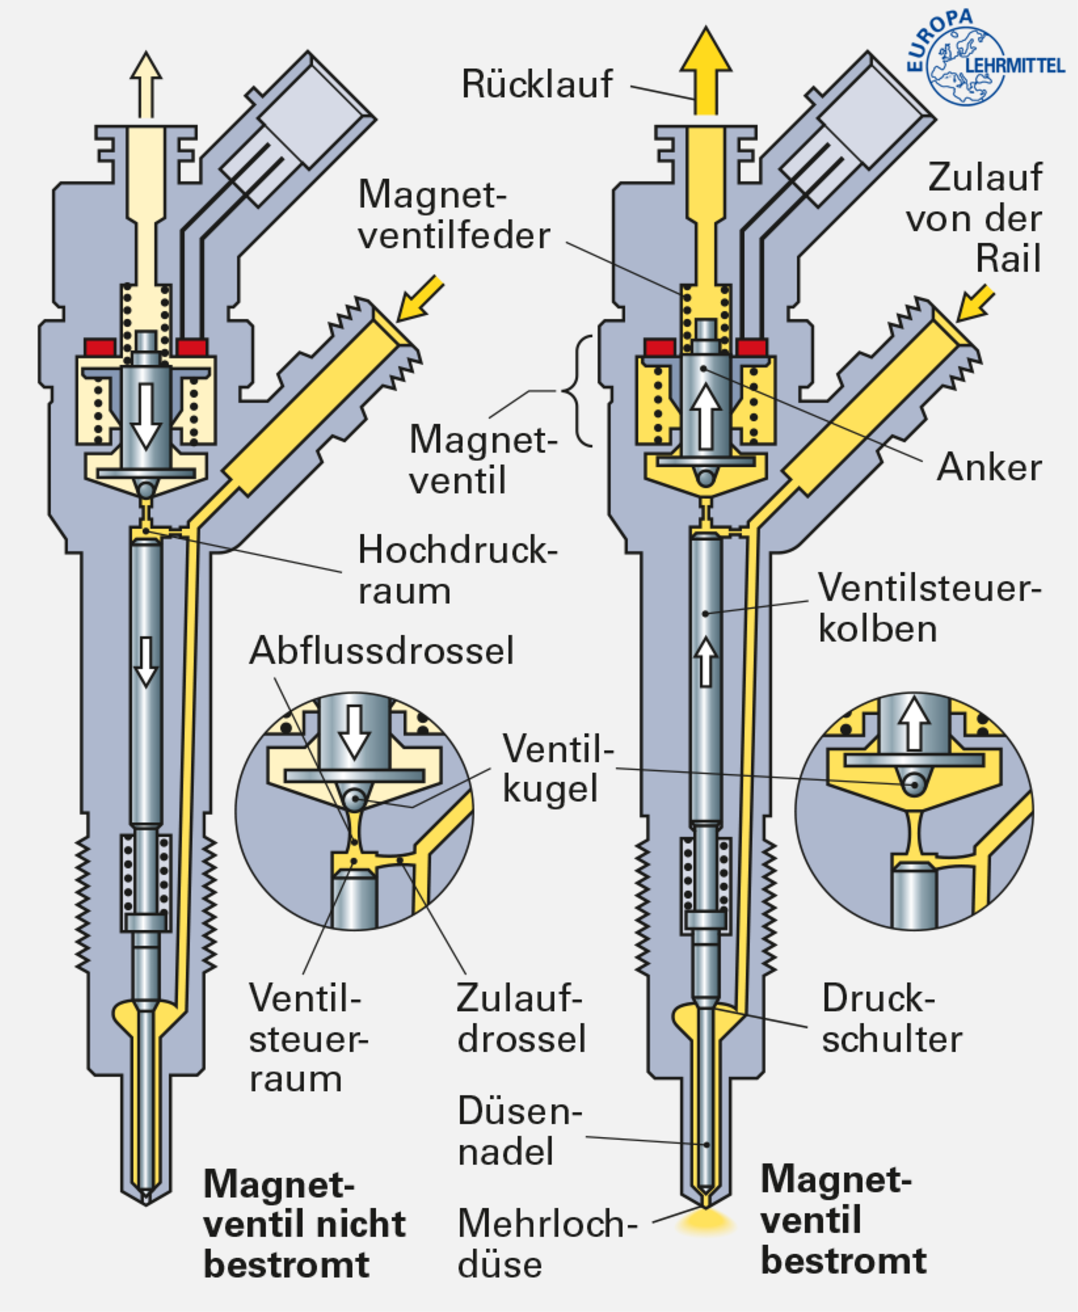
\includegraphics[width=0.4\textwidth]{images/CR/Wirkungsweise-Magnetventilinjektors.png}
\caption{Injektor mit Magnetventil, Quelle: Europa-Verlag SimKfz}
%\label{fig:}%% anpassen
\end{figure}

\begin{itemize}
\item
  \textbf{Magnetventil unbestromt - geschlossenen Zustand} dann wirkt im
  Ventilsteuerraum auf der Stirnfläche des Ventilsteuerkolbens und auf
  der Druckschulter der Düsennadel gleicher Kraftstoffkochdruck.
  Einspritzventil ist geschlossen.
\item
  \textbf{Magnetventil bestromt - geöffneten Zustand,} dann wird der
  Rücklauf geöffnet. Über die Ablaufdrossel entweicht mehr Kraftstoff,
  als über die Zulaufdrossel abfließen kann. Es kommt zum Druckabfall im
  Ventilsteuerraum. Der Druck auf die Druckschulter der Düsennadel kann
  die Düse öffnen. Düsennadel öffnet die Düse.
\end{itemize}

\textbf{Erklären Sie die Funktionsweise eines Injektors mit Piezoventil}

Piezoinjektoren erlauben hohe Schaltgeschwindigkeiten und damit viele
Teileinspritzungen.

\begin{itemize}
\item
  Piezo-Aktormodul wird bestromt und dehnt sich aus.
\item
  Über den hydraulischen Koppler findet eine Hubvergrößerung statt.
\item
  Öffnet das Servoventil und damit den Rücklauf.
\item
  Über die Ablaufdrossel fließt Kraftstoff aus dem Ventilsteuerraum ab.
\item
  Über die Zulaufdrossel kann weniger Kraftstoff in den Ventilsteuerraum
  zufließen. Es kommt zum Druckabfall.
\item
  Der Druck auf die Druckschulter der Düsennadel öffnet die Düsennadel
  des Injektors. Einspritzbeginn.
\end{itemize}


	%%%%%%%%%%%%%%%%%%%%%%%%%%%%%%%%%%%%%%%%%%%%%%%%%%%%%%%%%%%%%%%%%%
    % Bibliographie
    \printbibliography[category=cited]
\end{document}
